\section*{Глава 4\\Результаты расчётов}
\addcontentsline{toc}{section}{Глава 4. Результаты расчётов}
\setcounter{section}{4}
\setcounter{subsection}{0}
\setcounter{equation}{0}

\subsection{Верификация}

	В общем виде система линеных гиперболических уравнений \eqref{matrix_anisotropy_equation1} не решена и не доказана теорема существования её решения.
	Более того пока ещё не построено решение одномерной системы \eqref{norm_form}, получающейся после расщепления, для произвольного вида границы.
	Тем не менее после перехода к инвариантам система распадается на девять уравнений переноса, для которых известно аналитическое решение.
	Воспользуемся этим решением для проверки численного метода в простейшем случае \textbf{P} и \textbf{S} волн.

\subsubsection{P, S - волны}

	\textit{P-волной} называется продольная упругая волна, т.е. волна у которой вектор распространения параллелен вектору поляризации.
	\textit{S-волна} -- поперечная упругая волна. Для нёё вектор распространения перпендикулярен вектору поляризации.
	
	Рассмотрим, как задать P и S волны для уравнения:
\begin{equation}
	\label{norm_form_results}
	\frac{\partial\vec{u}}{\partial{t}}+\mathbf{A}_z\frac{\partial\vec{u}}{\partial{z}}=0.
\end{equation}
	
	Пусть материал будет \textit{ортотропным}, тогда матрица упругих постоянных будет выглядеть следующим образом:
\begin{align}
\label{orthorombic_tensor}
\left( \begin{array}{cccccccccccc}
c_{11} & c_{12} & c_{13} & 0 & 0 & 0 \\ 
c_{12} & c_{22} & c_{23} & 0 & 0 & 0 \\ 
c_{13} & c_{23} & c_{33} & 0 & 0 & 0 \\ 
0 & 0 & 0 & c_{44} & 0 & 0 \\ 
0 & 0 & 0 & 0 & c_{55} & 0 \\ 
0 & 0 & 0 & 0 & 0 & c_{66}
\end{array} \right){}
\end{align}	
	Собственные значения для матрицы $\mathbf{A}_z$ в таком случае имеют вид:	
\begin{align}
	\left\{0,\;0,\;0,\;\sqrt{\frac{c_{33}}{\rho}},\;\sqrt{\frac{c_{44}}{\rho}},\;\sqrt{\frac{c_{55}}{\rho}},\;-\sqrt{\frac{c_{33}}{\rho}},\;-\sqrt{\frac{c_{44}}{\rho}},\;-\sqrt{\frac{c_{55}}{\rho}}\right\}.
\end{align}
	Инварианты Римана для уравнения \eqref{norm_form_results} можно записать $\vec{r} = \mathbf{\Omega}_z\vec{u}$ или покомпонентно:
\begin{align}
\label{Z_invariants}
\vec{r} =
\left( \begin{array}{cccccccccccc}
0 & 0 & 0 & 1 & 0 & 0 & 0 & 0 & -\frac{c_{13}}{c_{33}} \\ 
0 & 0 & 0 & 0 & 1 & 0 & 0 & 0 & 0 \\ 
0 & 0 & 0 & 0 & 0 & 0 & 1 & 0 & -\frac{c_{23}}{c_{33}} \\ 
0 & 0 & -\sqrt{c_{33}\rho} & 0 & 0 & 0 & 0 & 0 & 1 \\ 
0 & -\sqrt{c_{44}\rho} & 0 & 0 & 0 & 0 & 0 & 1 & 0 \\
-\sqrt{c_{55}\rho} & 0 & 0 & 0 & 0 & 1 & 0 & 0 & 0 \\
0 & 0 & \sqrt{c_{33}\rho} & 0 & 0 & 0 & 0 & 0 & 1 \\ 
0 & \sqrt{c_{44}\rho} & 0 & 0 & 0 & 0 & 0 & 1 & 0 \\
\sqrt{c_{55}\rho} & 0 & 0 & 0 & 0 & 1 & 0 & 0 & 0
\end{array} \right)
\left( \begin{array}{cccccccccccc}
v_x \\
v_y \\
v_z \\
\sigma_{xx} \\
\sigma_{xy} \\
\sigma_{xz} \\
\sigma_{yy} \\
\sigma_{yz} \\
\sigma_{zz}
\end{array} \right).
\end{align}
	
	Для создания P-волны вдоль направления $Z$ следует занулить все инварианты кроме инварианта, соответствующего продольной волне, т.е. кроме строчки в \eqref{Z_invariants}, соответствующей собственному значению $-\sqrt{\frac{c_{33}}{\rho}}$ (знак минус выбран для удобства).
	Потребуем зануления всех инвариантов, кроме седьмой строчки:
\begin{align}	
	\label{p_cond}
	\left\{
		\begin{array}{cccccccccccc}
			c_{33}\sigma_{xx} = c_{13}\sigma_{zz} \\
			\sigma_{xy} = 0 \\
			c_{33}\sigma_{yy} = c_{23}\sigma_{zz} \\
			v_z\sqrt{c_{33}\rho} = \sigma_{zz} \\
			\pm v_y\sqrt{c_{44}\rho} = \sigma_{yz} \\
			\pm v_x\sqrt{c_{55}\rho} = \sigma_{xz}
		\end{array}
	\right.
\end{align}
	Задав начальные значения неизвестных в соответствии с \eqref{p_cond}, получим P-волну в этом направлении.
	
	Аналогично можно выписать соотношения, задающие S-волну для уравнения переноса \eqref{norm_form_results}.
	Скорость распространения поперечной волны вдоль оси $X$ будет $-\sqrt{\frac{c_{55}}{\rho}}$, занулив все инварианты кроме последней строчки в \eqref{Z_invariants}, получим:
\begin{align}	
	\label{s_cond1}
	\left\{
		\begin{array}{cccccccccccc}
			c_{33}\sigma_{xx} = c_{13}\sigma_{zz} \\
			\sigma_{xy} = 0 \\
			c_{33}\sigma_{yy} = c_{23}\sigma_{zz} \\
			\pm v_z\sqrt{c_{33}\rho} = \sigma_{zz} \\
			\pm v_y\sqrt{c_{44}\rho} = \sigma_{yz} \\
			v_x\sqrt{c_{55}\rho} = \sigma_{xz}
		\end{array}
	\right.
\end{align}

	И для поперечной S-волны для \eqref{norm_form_results} вдоль оси $Y$, распространяющейся со скоростью $-\sqrt{\frac{c_{44}}{\rho}}$ имеем:
\begin{align}	
	\label{s_cond2}
	\left\{
		\begin{array}{cccccccccccc}
			c_{33}\sigma_{xx} = c_{13}\sigma_{zz} \\
			\sigma_{xy} = 0 \\
			c_{33}\sigma_{yy} = c_{23}\sigma_{zz} \\
			\pm v_z\sqrt{c_{33}\rho} = \sigma_{zz} \\
			v_y\sqrt{c_{44}\rho} = \sigma_{yz} \\
			\pm v_x\sqrt{c_{55}\rho} = \sigma_{xz}
		\end{array}
	\right.
\end{align}

	Для остальных уравнений вида \eqref{norm_form_results} расщеплённой системы P и S волны задаются по аналогии.
	
\subsubsection{Результаты тестовых расчётов}

	В процессе выполнения работы была произведена модификация пакета программ, предназначенного для численного моделирования динамических процессов распространения механических деформаций в твёрдых телах сеточно-характеристическим методом с явным выделением контакта, для поддержки расчёта анизотропных тел.

	Для проверки созданной модификации были написаны функциональные тесты, сравнивающие численное решение распространения P и S волн в одномерной проекции, а также таски (задания расчётов), создающие эти волны.
	
	За модельный был взят трансверсально-изотропный материал с матрицей упругих постоянных:
\begin{align}
\label{veryfication_mat}
\left( \begin{array}{cccccccccccc}
90000 & 70000 & 17500 & 0 & 0 & 0 \\ 
70000 & 90000 & 17500 & 0 & 0 & 0 \\ 
17500 & 17500 & 22500 & 0 & 0 & 0 \\ 
0 & 0 & 0 & 10000 & 0 & 0 \\ 
0 & 0 & 0 & 0 & 10000 & 0 \\ 
0 & 0 & 0 & 0 & 0 & 10000
\end{array} \right),
\end{align}	
	и условной плотностью равной:
\begin{equation}
	\rho = 1.
\end{equation}
	Все указанные числа обезразмерены.
	Единицу измерения им можно придать задав единицу измерения времени (шаг метода) и единицу измерения длины (размер тела).

	Общий трёхмерный вид всех P и S возмущений представлен на рисунке снизу.
\begin{figure}[H]
\centerline{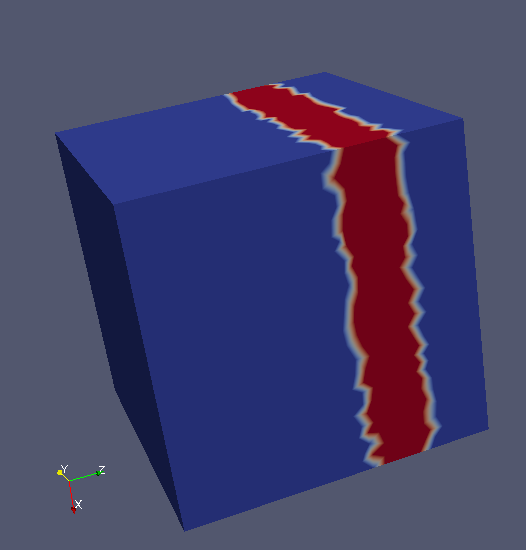
\includegraphics[width=0.4\textwidth]{png/veryfication/p-wave-view.png}}
\caption{Общий трёхмерный вид всех P, S волн. Цветовой гаммой выделена амплитуда скорости.}
\label{pic:p-wave-view}
\end{figure}
	
	Ниже представлены рисунки сравнения численного и аналитического решений для P и S волн уравнения переноса с матрицами $\mathbf{A}_x$, $\mathbf{A}_z$ на различных мелкостях сетки.
	Плоскость $XY$ изотропна, поэтому в ней можно провести проверку в одном направлении.
\begin{figure}[H]
\begin{subfigure}[b]{0.5\textwidth}
\centering
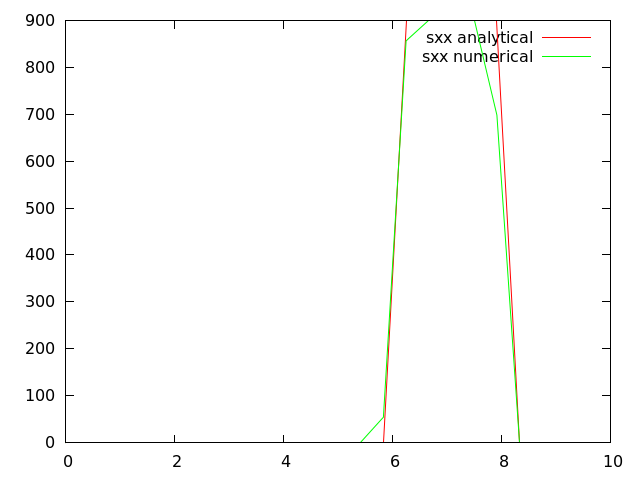
\includegraphics[width=0.75\textwidth]{png/veryfication/0.8/p-wave-along-x0.png}
\caption{Начальное состояние}
\end{subfigure}
\begin{subfigure}[b]{0.5\textwidth}
\centering
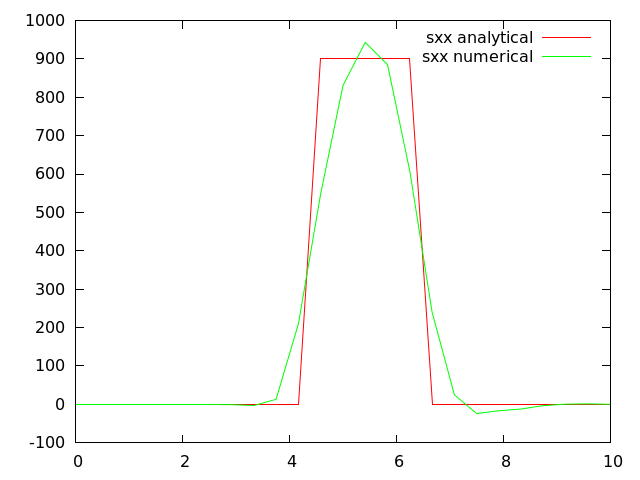
\includegraphics[width=0.75\textwidth]{png/veryfication/0.8/p-wave-along-x5.png}
\caption{5-ый шаг}
\end{subfigure}
\begin{subfigure}[b]{0.5\textwidth}
\centering
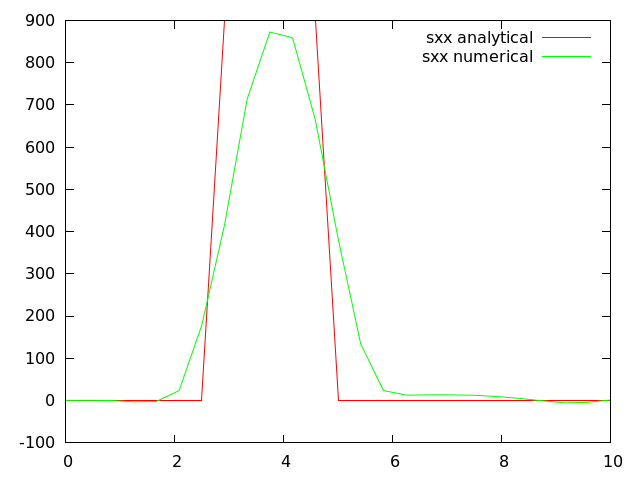
\includegraphics[width=0.75\textwidth]{png/veryfication/0.8/p-wave-along-x10.png}
\caption{10-ый шаг}
\end{subfigure}
\begin{subfigure}[b]{0.5\textwidth}
\centering
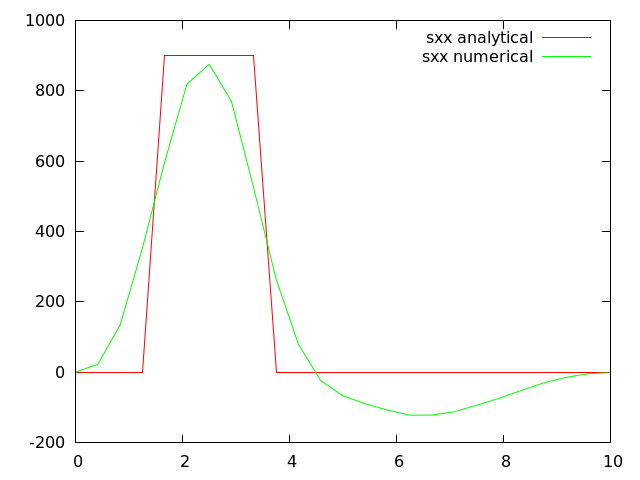
\includegraphics[width=0.75\textwidth]{png/veryfication/0.8/p-wave-along-x15.png}
\caption{15-ый шаг}
\end{subfigure}
\caption{Распространение P-волны вдоль оси $X$. Показана $\sigma_{xx}$ компонента. Размер тетраэдра -- 0.8, шаг по времени -- 0.001025. }
\label{pic:p_wave_along_x8}
\end{figure}

\begin{figure}[H]
\begin{subfigure}[b]{0.5\textwidth}
\centering
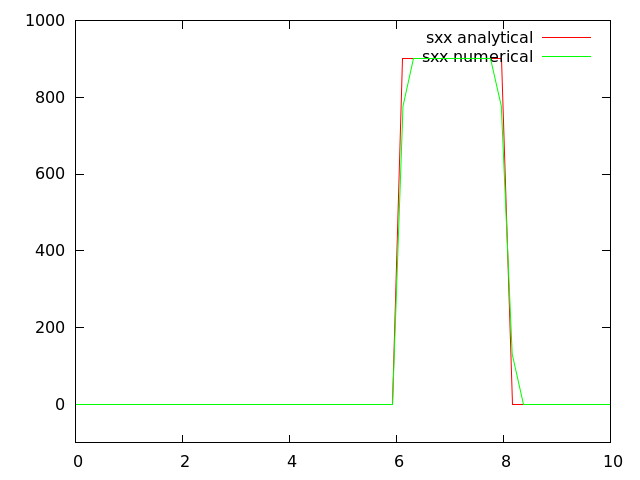
\includegraphics[width=0.75\textwidth]{png/veryfication/0.4/p-wave-along-x0.png}
\caption{Начальное состояние}
\end{subfigure}
\begin{subfigure}[b]{0.5\textwidth}
\centering
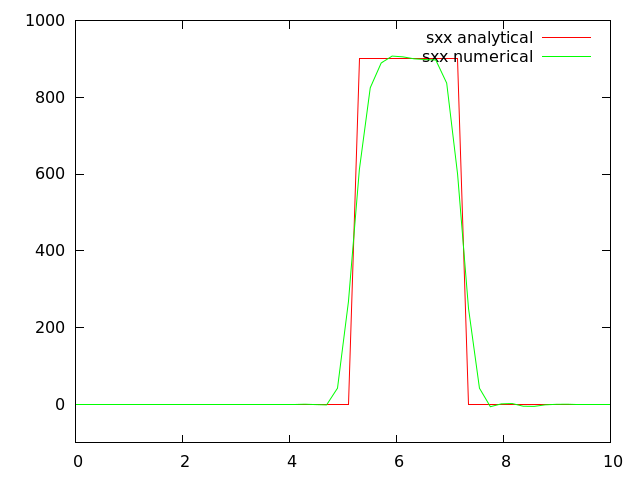
\includegraphics[width=0.75\textwidth]{png/veryfication/0.4/p-wave-along-x5.png}
\caption{5-ый шаг}
\end{subfigure}
\begin{subfigure}[b]{0.5\textwidth}
\centering
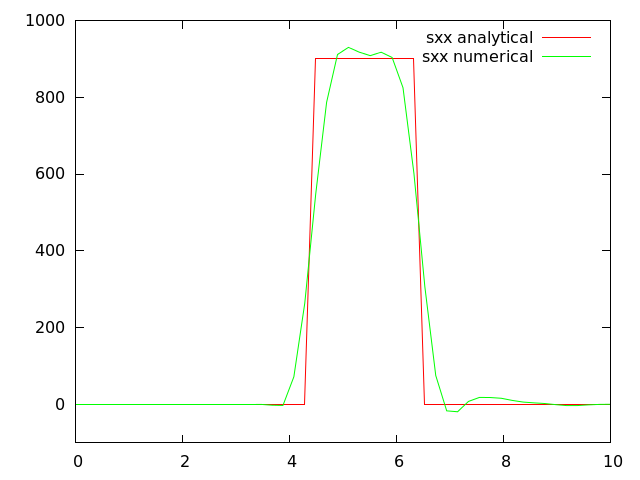
\includegraphics[width=0.75\textwidth]{png/veryfication/0.4/p-wave-along-x10.png}
\caption{10-ый шаг}
\end{subfigure}
\begin{subfigure}[b]{0.5\textwidth}
\centering
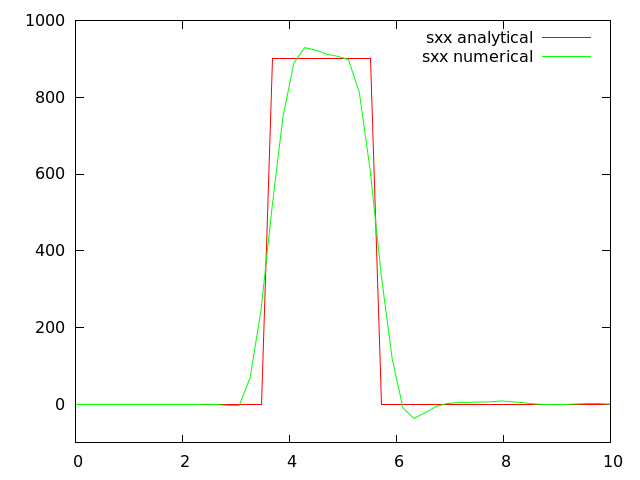
\includegraphics[width=0.75\textwidth]{png/veryfication/0.4/p-wave-along-x15.png}
\caption{15-ый шаг}
\end{subfigure}
\caption{Распространение P-волны вдоль оси $X$. Показана $\sigma_{xx}$ компонента. Размер тетраэдра -- 0.4, шаг по времени -- 0.000533. }
\label{pic:p_wave_along_x4}
\end{figure}

\begin{figure}[H]
\begin{subfigure}[b]{0.5\textwidth}
\centering
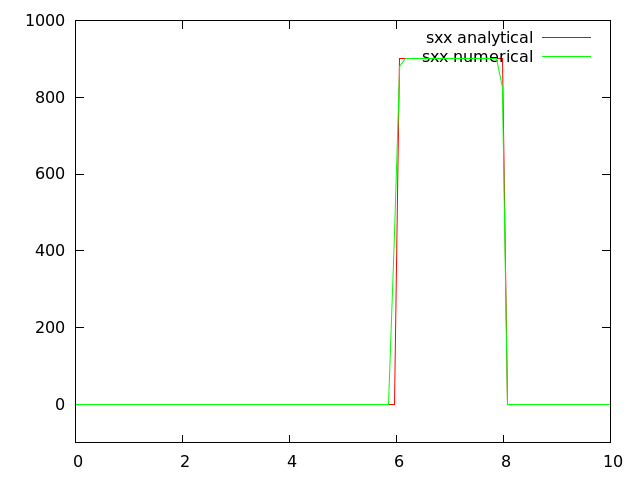
\includegraphics[width=0.75\textwidth]{png/veryfication/0.2/p-wave-along-x0.png}
\caption{Начальное состояние}
\end{subfigure}
\begin{subfigure}[b]{0.5\textwidth}
\centering
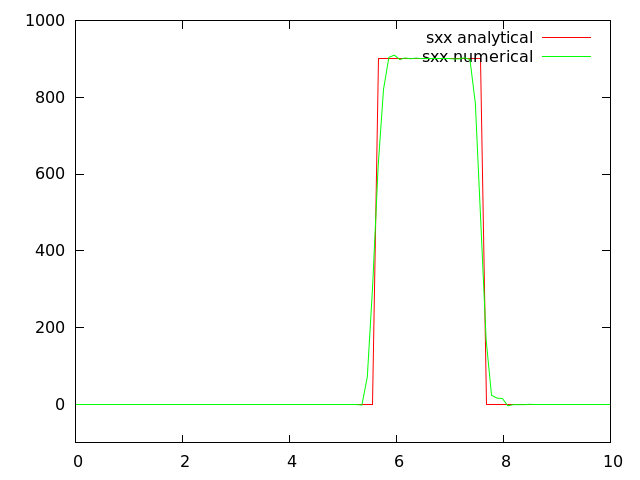
\includegraphics[width=0.75\textwidth]{png/veryfication/0.2/p-wave-along-x5.png}
\caption{5-ый шаг}
\end{subfigure}
\begin{subfigure}[b]{0.5\textwidth}
\centering
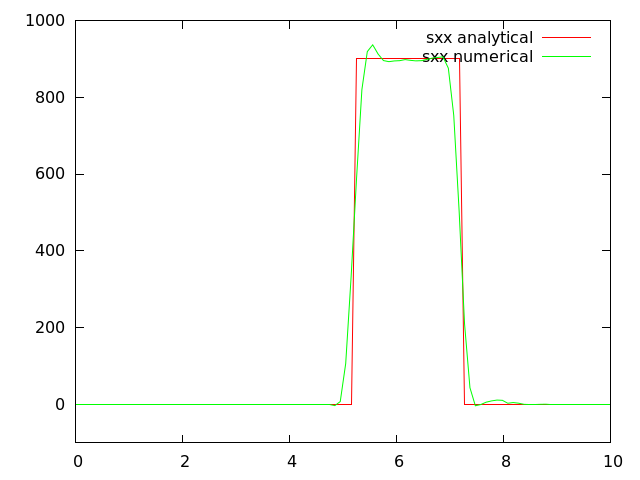
\includegraphics[width=0.75\textwidth]{png/veryfication/0.2/p-wave-along-x10.png}
\caption{10-ый шаг}
\end{subfigure}
\begin{subfigure}[b]{0.5\textwidth}
\centering
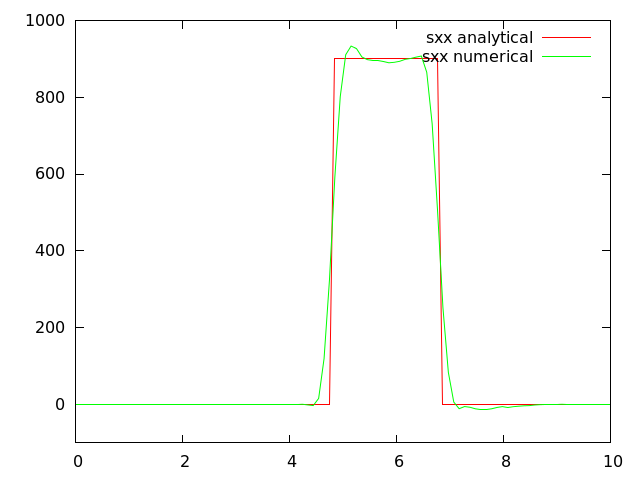
\includegraphics[width=0.75\textwidth]{png/veryfication/0.2/p-wave-along-x15.png}
\caption{15-ый шаг}
\end{subfigure}
\caption{Распространение P-волны вдоль оси $X$. Показана $\sigma_{xx}$ компонента. Размер тетраэдра -- 0.2, шаг по времени -- 0.000269. }
\label{pic:p_wave_along_x2}
\end{figure}

\begin{figure}[H]
\begin{subfigure}[b]{0.5\textwidth}
\centering
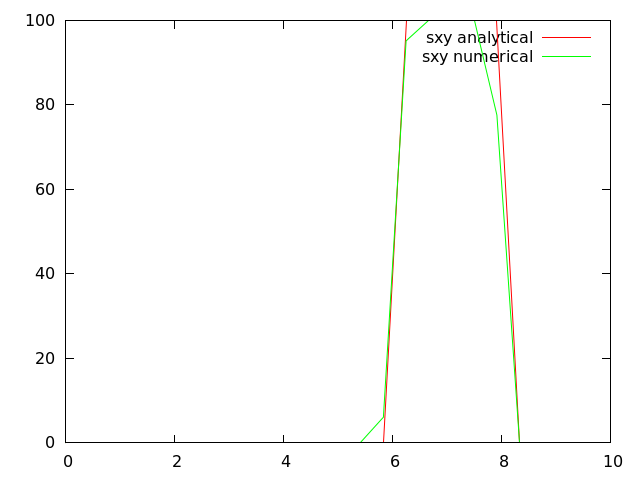
\includegraphics[width=0.75\textwidth]{png/veryfication/0.8/s-wave-along-x0.png}
\caption{Начальное состояние}
\end{subfigure}
\begin{subfigure}[b]{0.5\textwidth}
\centering
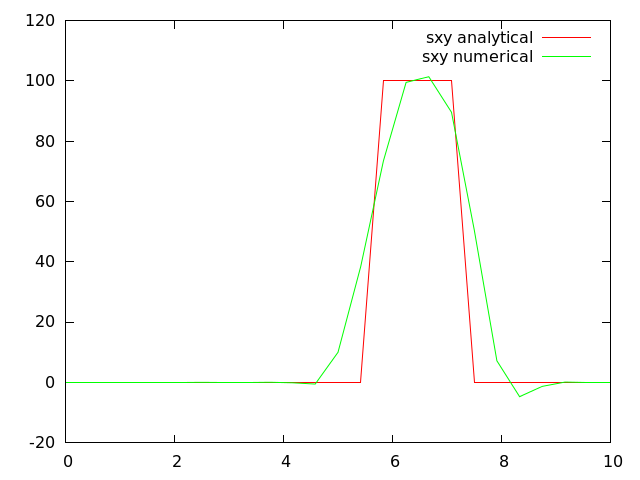
\includegraphics[width=0.75\textwidth]{png/veryfication/0.8/s-wave-along-x5.png}
\caption{5-ый шаг}
\end{subfigure}
\begin{subfigure}[b]{0.5\textwidth}
\centering
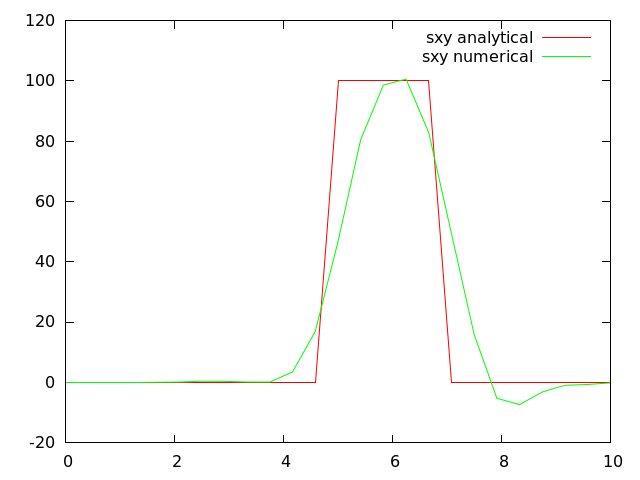
\includegraphics[width=0.75\textwidth]{png/veryfication/0.8/s-wave-along-x10.png}
\caption{10-ый шаг}
\end{subfigure}
\begin{subfigure}[b]{0.5\textwidth}
\centering
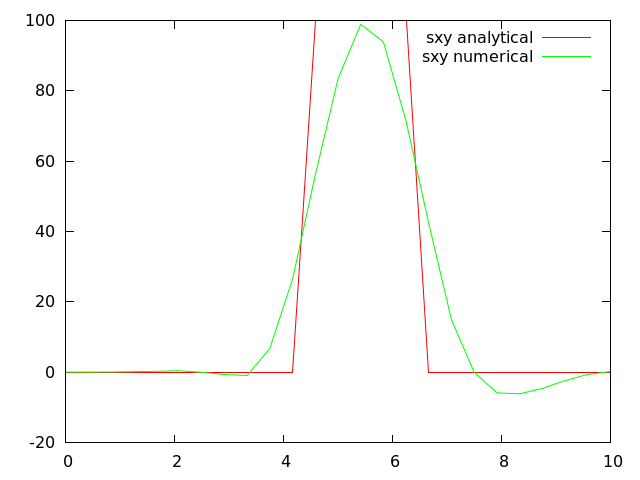
\includegraphics[width=0.75\textwidth]{png/veryfication/0.8/s-wave-along-x15.png}
\caption{15-ый шаг}
\end{subfigure}
\caption{Распространение S-волны вдоль оси $X$. Показана $\sigma_{xy}$ компонента. Размер тетраэдра -- 0.8, шаг по времени -- 0.001025. }
\label{pic:s_wave_along_x8}
\end{figure}

\begin{figure}[H]
\begin{subfigure}[b]{0.5\textwidth}
\centering
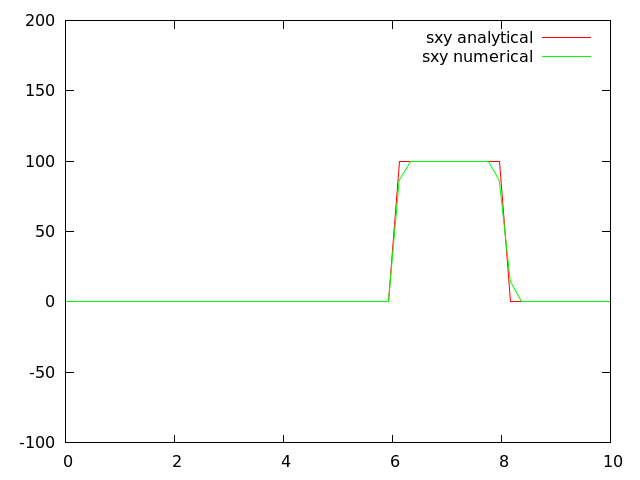
\includegraphics[width=0.75\textwidth]{png/veryfication/0.4/s-wave-along-x0.png}
\caption{Начальное состояние}
\end{subfigure}
\begin{subfigure}[b]{0.5\textwidth}
\centering
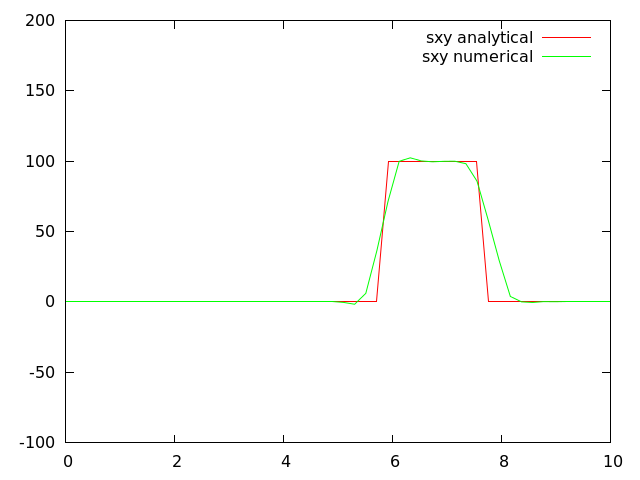
\includegraphics[width=0.75\textwidth]{png/veryfication/0.4/s-wave-along-x5.png}
\caption{5-ый шаг}
\end{subfigure}
\begin{subfigure}[b]{0.5\textwidth}
\centering
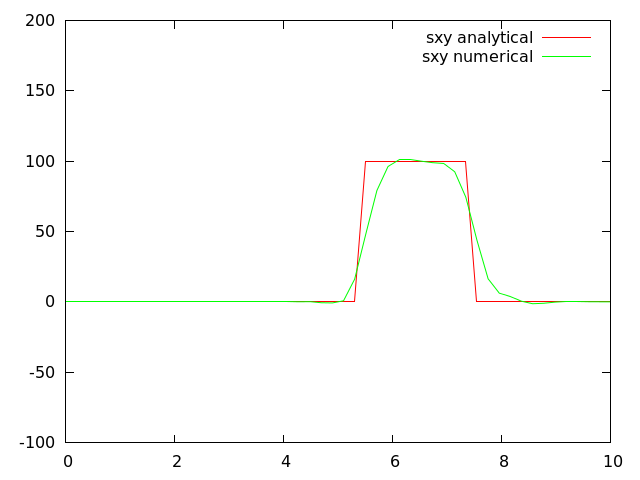
\includegraphics[width=0.75\textwidth]{png/veryfication/0.4/s-wave-along-x10.png}
\caption{10-ый шаг}
\end{subfigure}
\begin{subfigure}[b]{0.5\textwidth}
\centering
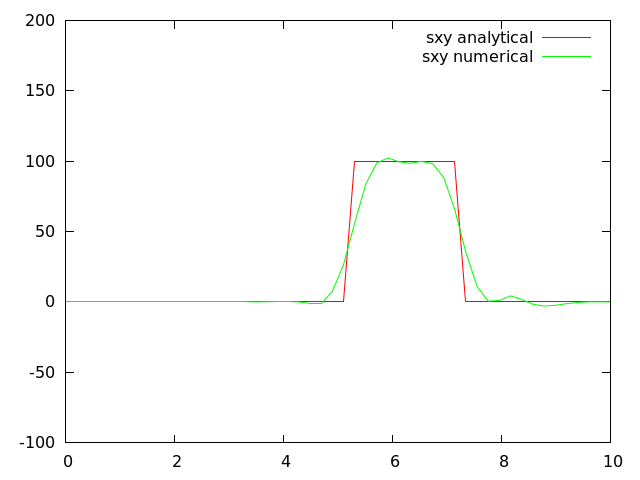
\includegraphics[width=0.75\textwidth]{png/veryfication/0.4/s-wave-along-x15.png}
\caption{15-ый шаг}
\end{subfigure}
\caption{Распространение S-волны вдоль оси $X$. Показана $\sigma_{xy}$ компонента. Размер тетраэдра -- 0.4, шаг по времени -- 0.000533. }
\label{pic:s_wave_along_x4}
\end{figure}

\begin{figure}[H]
\begin{subfigure}[b]{0.5\textwidth}
\centering
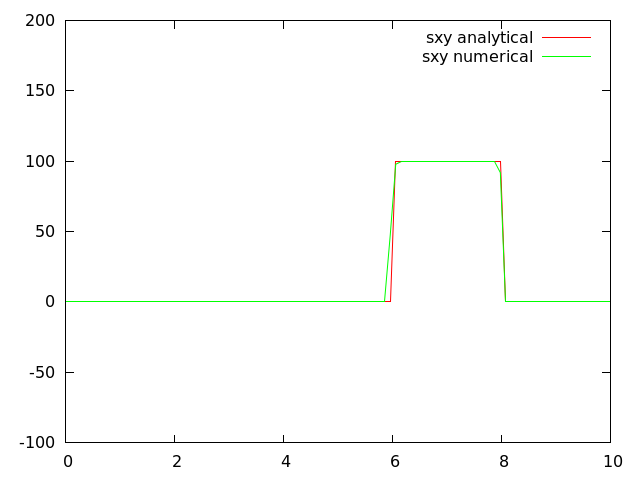
\includegraphics[width=0.75\textwidth]{png/veryfication/0.2/s-wave-along-x0.png}
\caption{Начальное состояние}
\end{subfigure}
\begin{subfigure}[b]{0.5\textwidth}
\centering
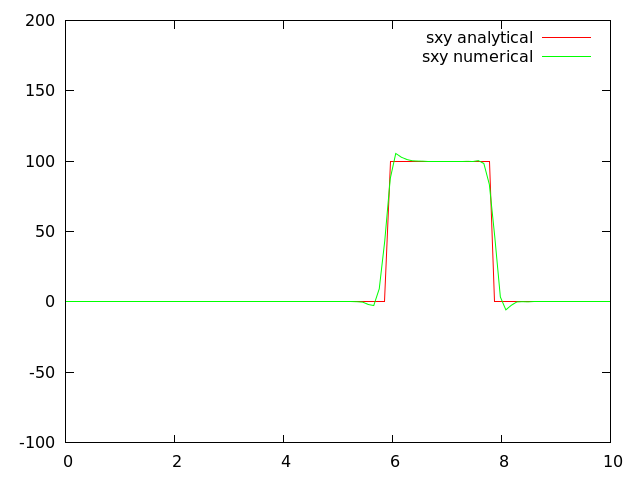
\includegraphics[width=0.75\textwidth]{png/veryfication/0.2/s-wave-along-x5.png}
\caption{5-ый шаг}
\end{subfigure}
\begin{subfigure}[b]{0.5\textwidth}
\centering
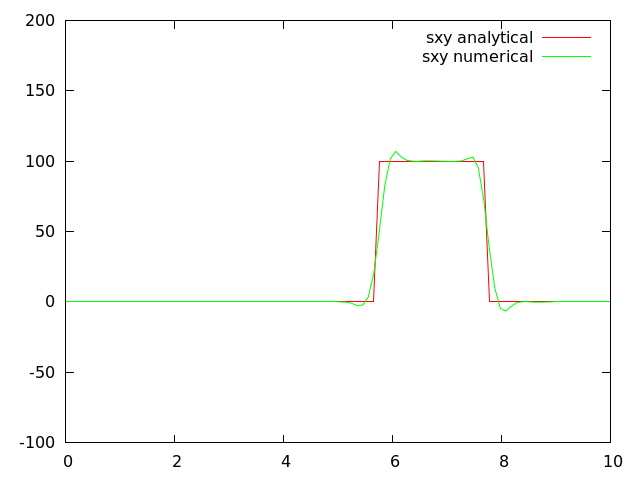
\includegraphics[width=0.75\textwidth]{png/veryfication/0.2/s-wave-along-x10.png}
\caption{10-ый шаг}
\end{subfigure}
\begin{subfigure}[b]{0.5\textwidth}
\centering
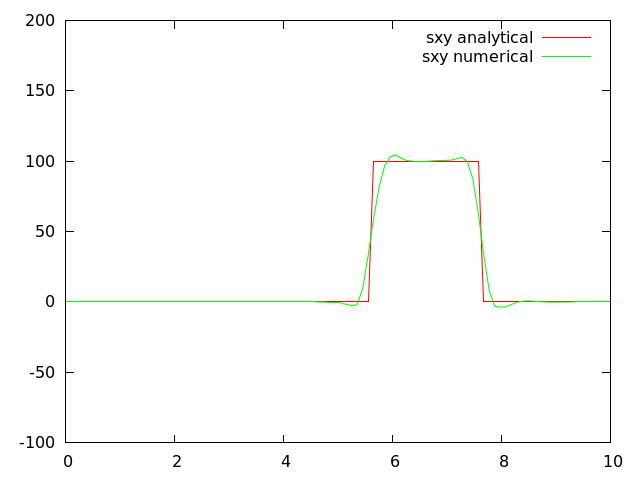
\includegraphics[width=0.75\textwidth]{png/veryfication/0.2/s-wave-along-x15.png}
\caption{15-ый шаг}
\end{subfigure}
\caption{Распространение S-волны вдоль оси $X$. Показана $\sigma_{xy}$ компонента. Размер тетраэдра -- 0.2, шаг по времени -- 0.000269. }
\label{pic:s_wave_along_x2}
\end{figure}

\begin{figure}[H]
\begin{subfigure}[b]{0.5\textwidth}
\centering
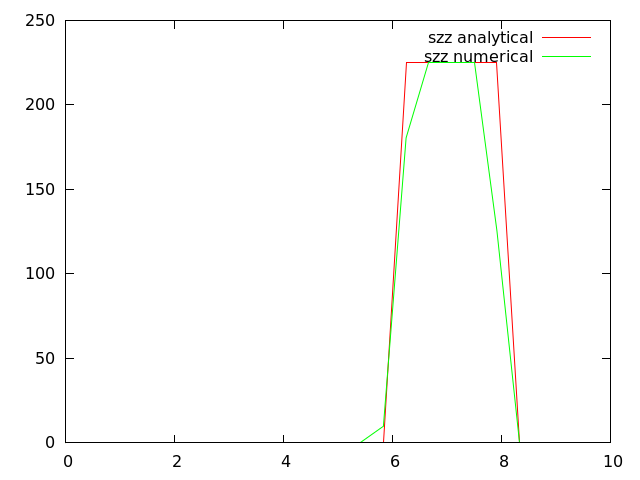
\includegraphics[width=0.75\textwidth]{png/veryfication/0.8/p-wave-along-z0.png}
\caption{Начальное состояние}
\end{subfigure}
\begin{subfigure}[b]{0.5\textwidth}
\centering
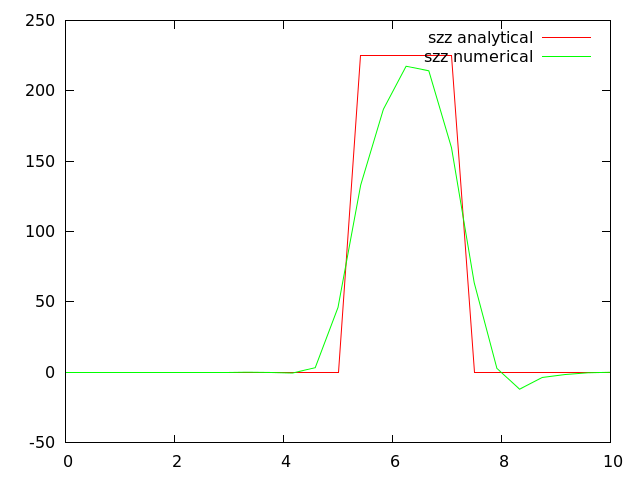
\includegraphics[width=0.75\textwidth]{png/veryfication/0.8/p-wave-along-z5.png}
\caption{5-ый шаг}
\end{subfigure}
\begin{subfigure}[b]{0.5\textwidth}
\centering
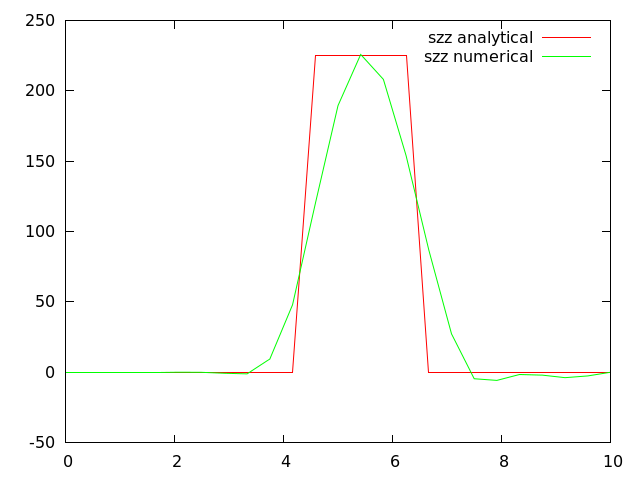
\includegraphics[width=0.75\textwidth]{png/veryfication/0.8/p-wave-along-z10.png}
\caption{10-ый шаг}
\end{subfigure}
\begin{subfigure}[b]{0.5\textwidth}
\centering
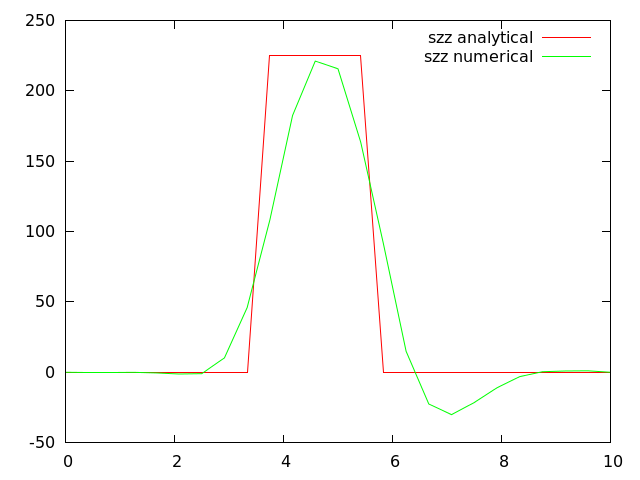
\includegraphics[width=0.75\textwidth]{png/veryfication/0.8/p-wave-along-z15.png}
\caption{15-ый шаг}
\end{subfigure}
\caption{Распространение P-волны вдоль оси $Z$. Показана $\sigma_{zz}$ компонента. Размер тетраэдра -- 0.8, шаг по времени -- 0.001025. }
\label{pic:p_wave_along_z8}
\end{figure}

\begin{figure}[H]
\begin{subfigure}[b]{0.5\textwidth}
\centering
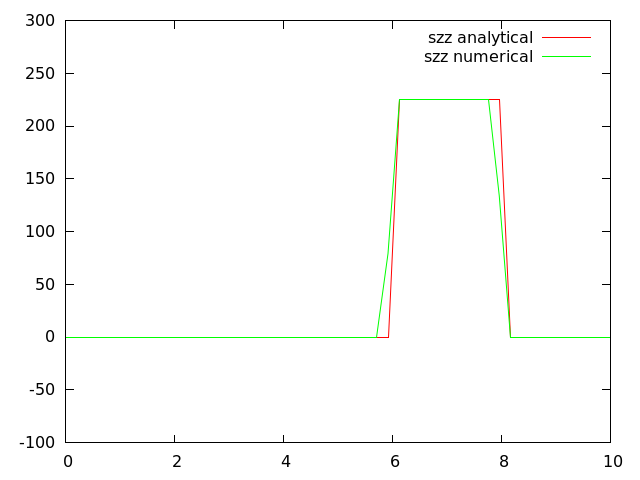
\includegraphics[width=0.75\textwidth]{png/veryfication/0.4/p-wave-along-z0.png}
\caption{Начальное состояние}
\end{subfigure}
\begin{subfigure}[b]{0.5\textwidth}
\centering
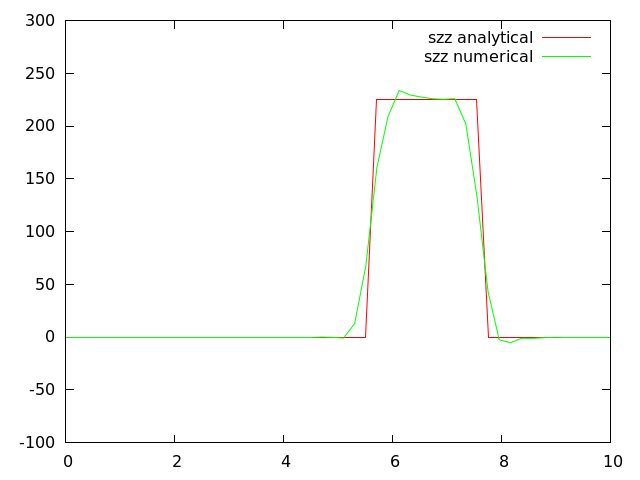
\includegraphics[width=0.75\textwidth]{png/veryfication/0.4/p-wave-along-z5.png}
\caption{5-ый шаг}
\end{subfigure}
\begin{subfigure}[b]{0.5\textwidth}
\centering
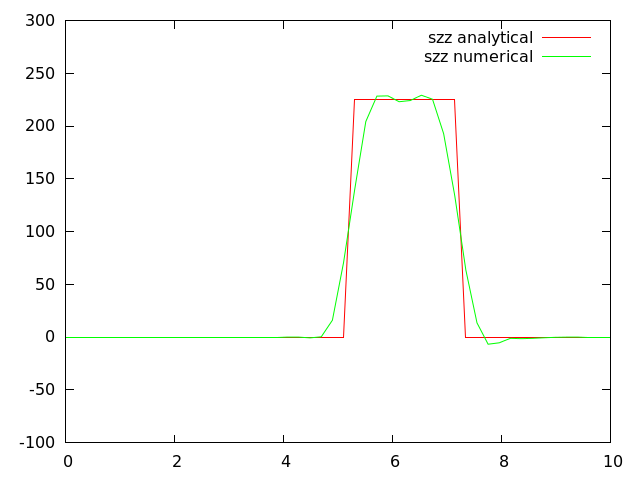
\includegraphics[width=0.75\textwidth]{png/veryfication/0.4/p-wave-along-z10.png}
\caption{10-ый шаг}
\end{subfigure}
\begin{subfigure}[b]{0.5\textwidth}
\centering
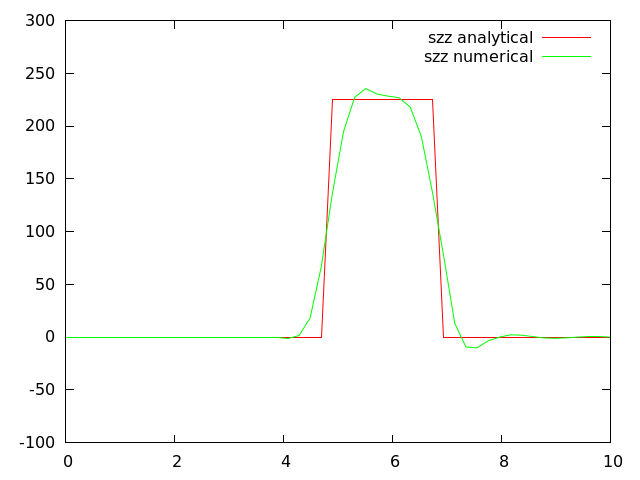
\includegraphics[width=0.75\textwidth]{png/veryfication/0.4/p-wave-along-z15.png}
\caption{15-ый шаг}
\end{subfigure}
\caption{Распространение P-волны вдоль оси $Z$. Показана $\sigma_{zz}$ компонента. Размер тетраэдра -- 0.4, шаг по времени -- 0.000533. }
\label{pic:p_wave_along_z4}
\end{figure}

\begin{figure}[H]
\begin{subfigure}[b]{0.5\textwidth}
\centering
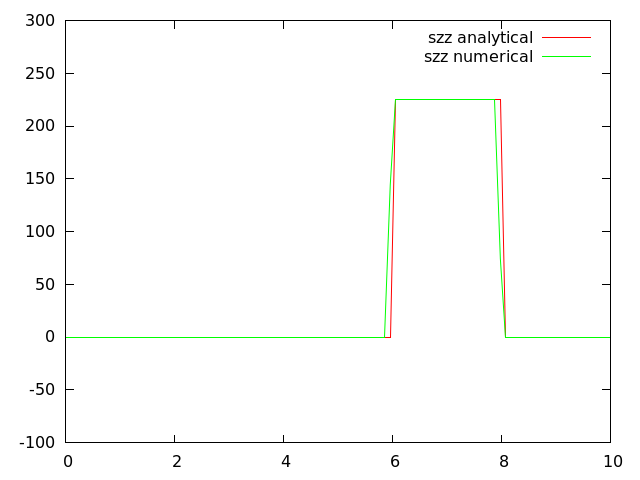
\includegraphics[width=0.75\textwidth]{png/veryfication/0.2/p-wave-along-z0.png}
\caption{Начальное состояние}
\end{subfigure}
\begin{subfigure}[b]{0.5\textwidth}
\centering
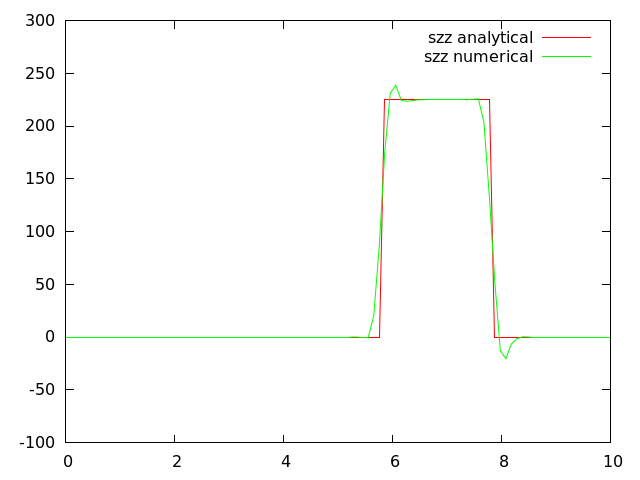
\includegraphics[width=0.75\textwidth]{png/veryfication/0.2/p-wave-along-z5.png}
\caption{5-ый шаг}
\end{subfigure}
\begin{subfigure}[b]{0.5\textwidth}
\centering
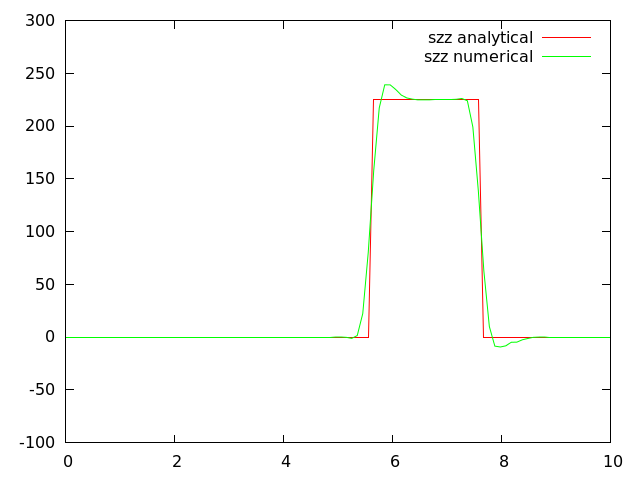
\includegraphics[width=0.75\textwidth]{png/veryfication/0.2/p-wave-along-z10.png}
\caption{10-ый шаг}
\end{subfigure}
\begin{subfigure}[b]{0.5\textwidth}
\centering
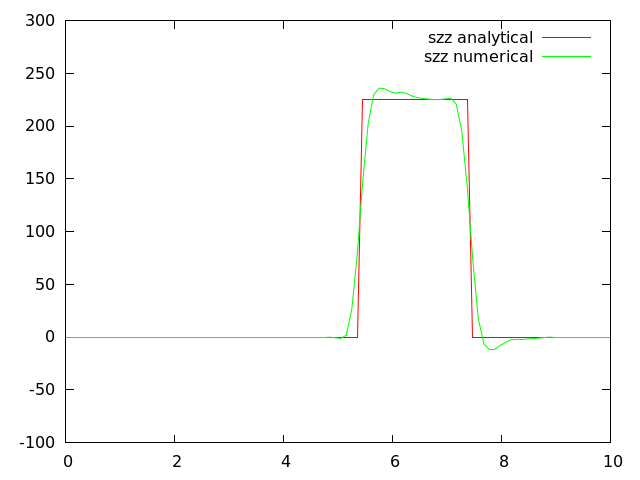
\includegraphics[width=0.75\textwidth]{png/veryfication/0.2/p-wave-along-z15.png}
\caption{15-ый шаг}
\end{subfigure}
\caption{Распространение P-волны вдоль оси $Z$. Показана $\sigma_{zz}$ компонента. Размер тетраэдра -- 0.2, шаг по времени -- 0.000269. }
\label{pic:p_wave_along_z2}
\end{figure}

\begin{figure}[H]
\begin{subfigure}[b]{0.5\textwidth}
\centering
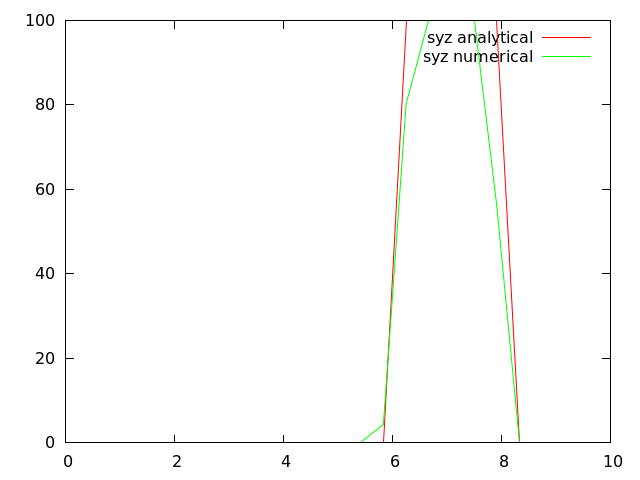
\includegraphics[width=0.75\textwidth]{png/veryfication/0.8/s-wave-along-z0.png}
\caption{Начальное состояние}
\end{subfigure}
\begin{subfigure}[b]{0.5\textwidth}
\centering
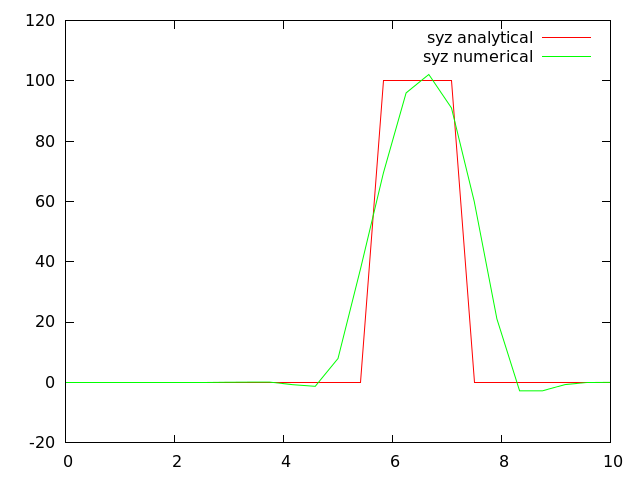
\includegraphics[width=0.75\textwidth]{png/veryfication/0.8/s-wave-along-z5.png}
\caption{5-ый шаг}
\end{subfigure}
\begin{subfigure}[b]{0.5\textwidth}
\centering
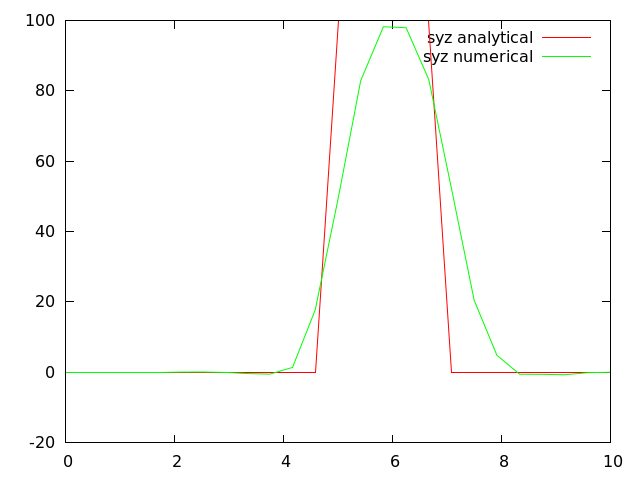
\includegraphics[width=0.75\textwidth]{png/veryfication/0.8/s-wave-along-z10.png}
\caption{10-ый шаг}
\end{subfigure}
\begin{subfigure}[b]{0.5\textwidth}
\centering
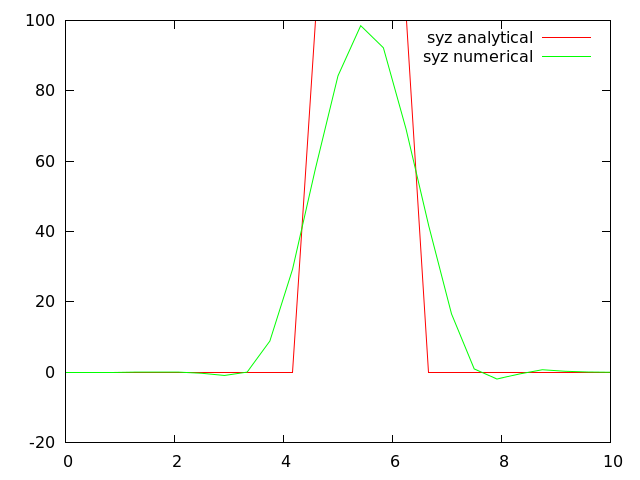
\includegraphics[width=0.75\textwidth]{png/veryfication/0.8/s-wave-along-z15.png}
\caption{15-ый шаг}
\end{subfigure}
\caption{Распространение S-волны вдоль оси $Z$. Показана $\sigma_{yz}$ компонента. Размер тетраэдра -- 0.8, шаг по времени -- 0.001025. }
\label{pic:s_wave_along_z8}
\end{figure}

\begin{figure}[H]
\begin{subfigure}[b]{0.5\textwidth}
\centering
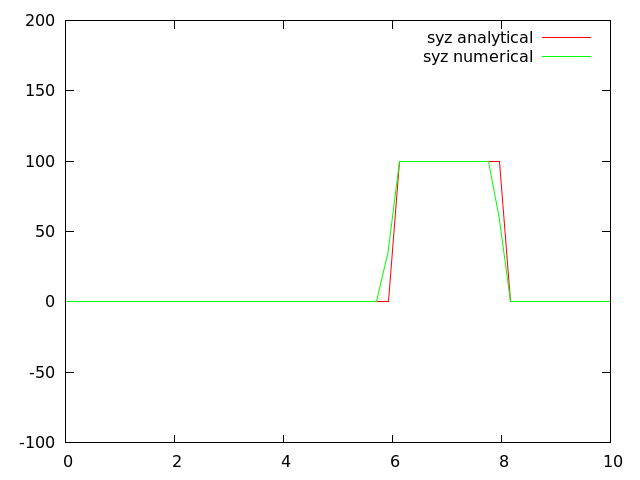
\includegraphics[width=0.75\textwidth]{png/veryfication/0.4/s-wave-along-z0.png}
\caption{Начальное состояние}
\end{subfigure}
\begin{subfigure}[b]{0.5\textwidth}
\centering
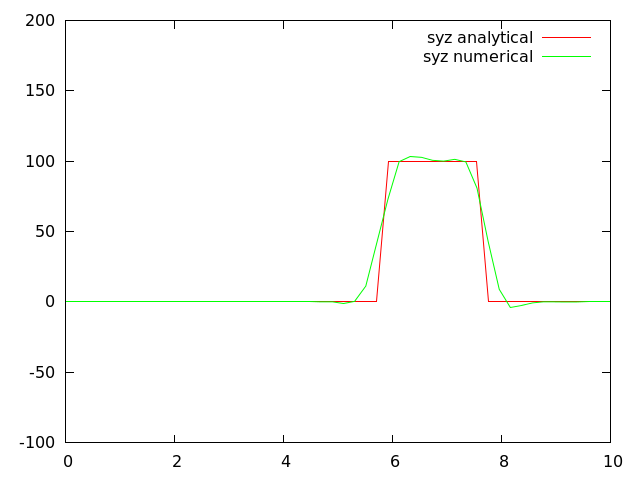
\includegraphics[width=0.75\textwidth]{png/veryfication/0.4/s-wave-along-z5.png}
\caption{5-й шаг}
\end{subfigure}
\begin{subfigure}[b]{0.5\textwidth}
\centering
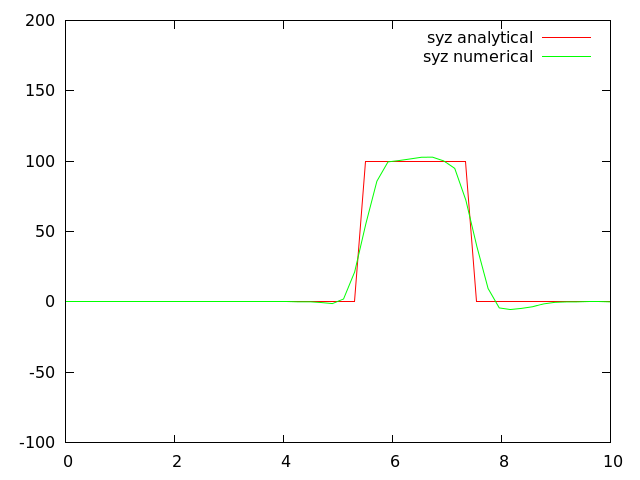
\includegraphics[width=0.75\textwidth]{png/veryfication/0.4/s-wave-along-z10.png}
\caption{10-й шаг}
\end{subfigure}
\begin{subfigure}[b]{0.5\textwidth}
\centering
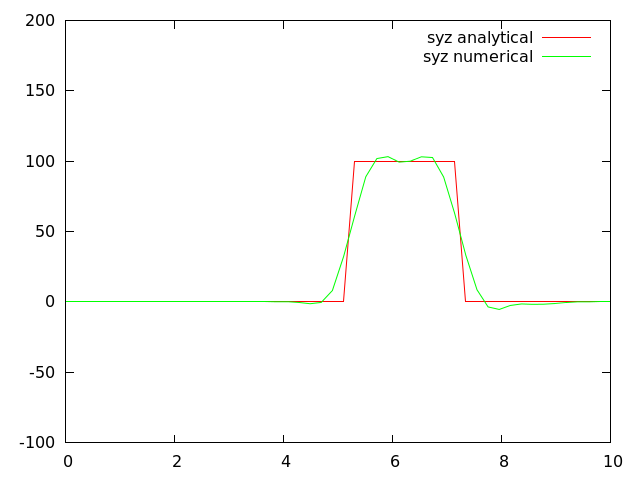
\includegraphics[width=0.75\textwidth]{png/veryfication/0.4/s-wave-along-z15.png}
\caption{15-й шаг}
\end{subfigure}
\caption{Распространение S-волны вдоль оси $Z$. Показана $\sigma_{yz}$ компонента. Размер тетраэдра -- 0.4, шаг по времени -- 0.000533. }
\label{pic:s_wave_along_z4}
\end{figure}

\begin{figure}[H]
\begin{subfigure}[b]{0.5\textwidth}
\centering
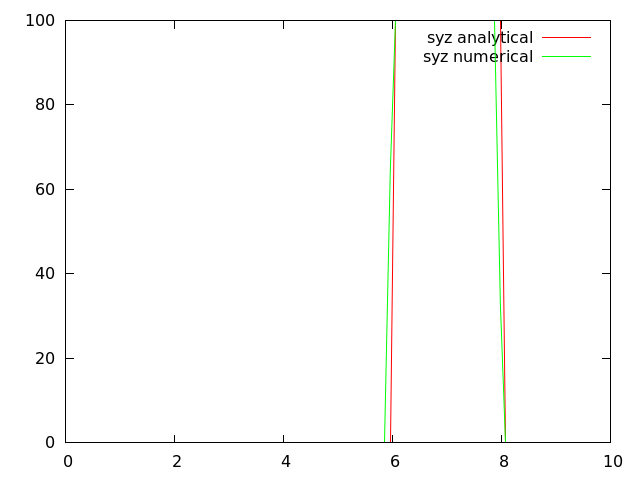
\includegraphics[width=0.75\textwidth]{png/veryfication/0.2/s-wave-along-z0.png}
\caption{Начальное состояние}
\end{subfigure}
\begin{subfigure}[b]{0.5\textwidth}
\centering
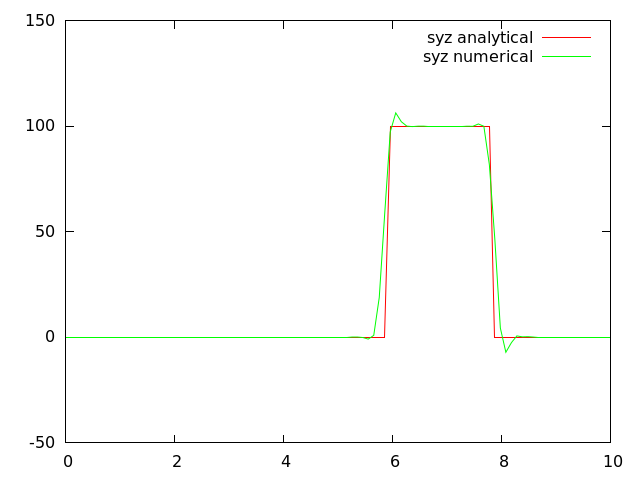
\includegraphics[width=0.75\textwidth]{png/veryfication/0.2/s-wave-along-z5.png}
\caption{5-ый шаг}
\end{subfigure}
\begin{subfigure}[b]{0.5\textwidth}
\centering
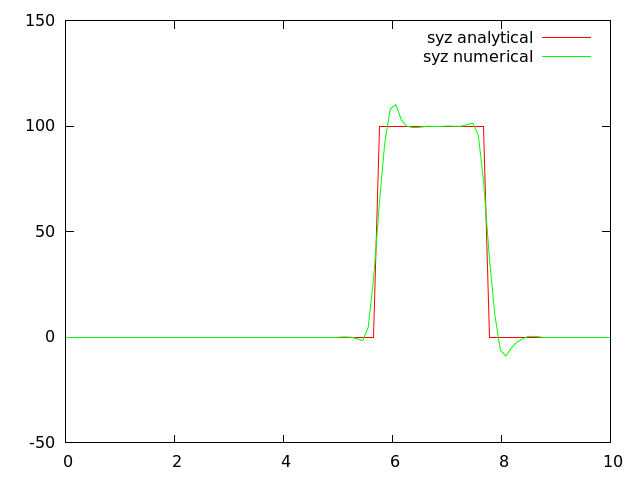
\includegraphics[width=0.75\textwidth]{png/veryfication/0.2/s-wave-along-z10.png}
\caption{10-ый шаг}
\end{subfigure}
\begin{subfigure}[b]{0.5\textwidth}
\centering
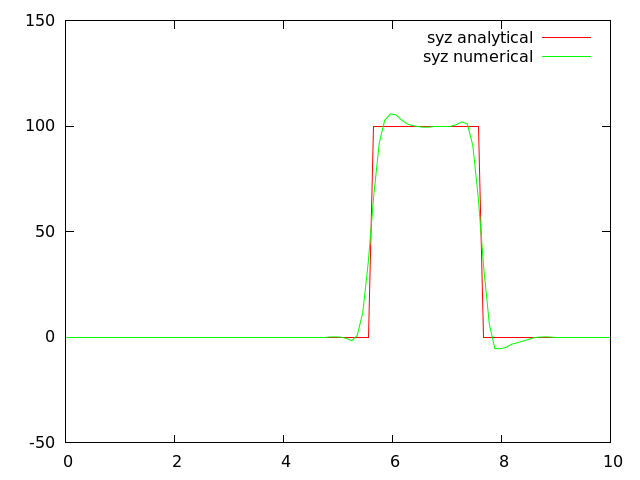
\includegraphics[width=0.75\textwidth]{png/veryfication/0.2/s-wave-along-z15.png}
\caption{15-ый шаг}
\end{subfigure}
\caption{Распространение S-волны вдоль оси $Z$. Показана $\sigma_{yz}$ компонента. Размер тетраэдра -- 0.2, шаг по времени -- 0.000269. }
\label{pic:s_wave_along_z2}
\end{figure}

	Из рисунков можно сделать вывод, что численные решения распространения P и S волн совпадают с их аналитическими аналогами с точностью до погрешности метода и аналитического приближения.
	Также из рисунков видно, что присутствует сходимость по пространству, однако определить её точное значение по этим данным невозможно, так как полученное значение будет сильно занижено, по сравнению с реальным, в силу грубого аналитического приближения трёхмерной задачи.

\subsection{Расчёт точечного взрыва в однородном теле}

	Был произведён расчёт точечного взрыва в изотропном и ортотропном телах.
	Ниже приведены плоские картинки для сравнения взрыва в изотропной и анизотропной средах.
	
	На Рис. \ref{pic:isotropic-explosion} показаны сферические волны модуля скорости среды в изотропном материале.
	На Рис. \ref{pic:anisotropic-explosion1} представлено то же самое, только в анизотропной среде.
	Вид фронта сферических волн здесь принимает форму эллипса, а также можно наблюдать распространение сдвиговых волн \cite{ogurtsov}, амплитуда которых максимальна на направлении, составляющем 45 градусов с осями.
	Эти волны -- существенное проявление анизотропии материала, в изотропном случае их нет.
	На Рис. \ref{pic:anisotropic-explosion2} изображено отражение волн в анизотропном случае.
	
\begin{figure}[H]
\centerline{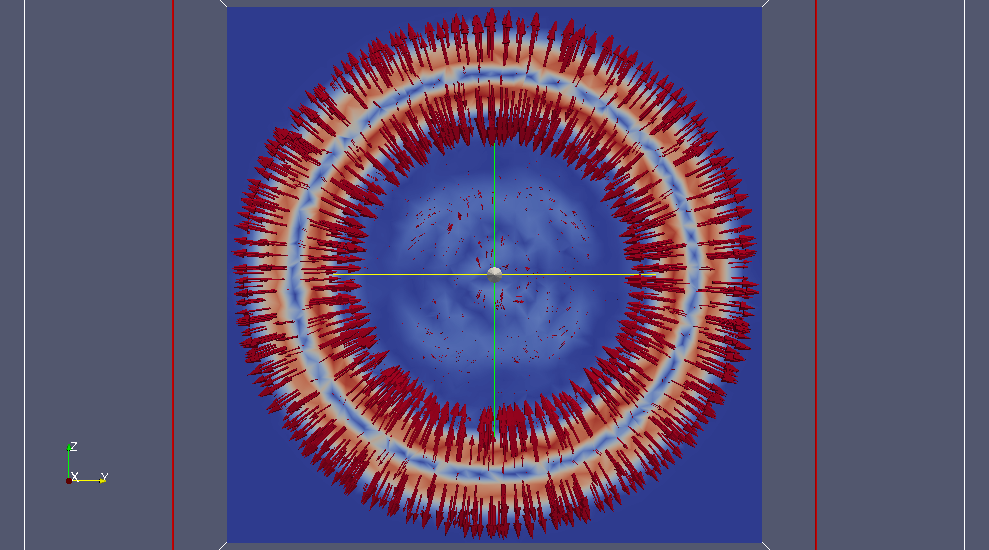
\includegraphics[width=0.75\textwidth]{png/dotted_explosion/exp_i_00.png}}
\caption{Точечный взрыв в изотропном теле. Плоский срез. Сферические волны амлитуды скорости.}
\label{pic:isotropic-explosion}
\end{figure}

\begin{figure}[H]
\centerline{\includegraphics[width=0.75\textwidth]{png/dotted_explosion/exp_ai_00.png}}
\caption{Точечный взрыв в анизотропном теле. Плоский срез. Сферические волны амлитуды скорости, а также видны сдвиговые волны рапространяющие под 45 градусов к осям.}
\label{pic:anisotropic-explosion1}
\end{figure}

\begin{figure}[H]
\centerline{\includegraphics[width=0.75\textwidth]{png/dotted_explosion/exp_ai_01.png}}
\caption{Точечный взрыв в анизотропном теле. Плоский срез. Отражение от границ.}
\label{pic:anisotropic-explosion2}
\end{figure}

\subsection{Расчёт двухслойной панели}

	Как уже было сказано, ПКМ -- многослойные анизотропные материалы, каждый субпакет которых включает в себя несколько слоев ортотропного материала, по-разному ориентированных вокруг оси укладки.
	Здесь мы рассмотрим расчёты динамического нагружения двухслойки, как некоторой минимальльной компоненты субпакета ПКМ.

	Под двухслойкой здесь мы понимаем два слоя трансверсально-изотропного материала, выделенные направления которых лежат в плоскости слоёв и составляют прямой угол друг с другом.
	Для начала используем тот же модельный материал, что мы использовали ранее:
\begin{align}
\label{model_mat}
\left( \begin{array}{cccccccccccc}
90000 & 70000 & 17500 & 0 & 0 & 0 \\ 
70000 & 90000 & 17500 & 0 & 0 & 0 \\ 
17500 & 17500 & 22500 & 0 & 0 & 0 \\ 
0 & 0 & 0 & 10000 & 0 & 0 \\ 
0 & 0 & 0 & 0 & 10000 & 0 \\ 
0 & 0 & 0 & 0 & 0 & 10000
\end{array} \right),
\end{align}	
\begin{equation}
	\rho = 1.
\end{equation}
	
	На рисунках снизу показано разделение на слои заданной области и вид начальной нагрузки -- удар прямоугольного профиля по поверхности верхнего слоя.	
\begin{figure}[H]
\begin{subfigure}[b]{0.5\textwidth}
\centering
\includegraphics[width=0.9\textwidth]{png/two-layers/view.png}
\caption{Разделение на слои.}
\end{subfigure}
\begin{subfigure}[b]{0.5\textwidth}
\centering
\includegraphics[width=0.9\textwidth]{png/two-layers/initial_view.png}
\caption{Вид начальной нагрузки.}
\end{subfigure}
\caption{Вид расчётной области.}
\label{pic:two_layers_view}
\end{figure}

	Ниже представлены изображения распространения волн в срезе четверти слоя.
	Тут отлично прослеживается анизотропия распростванения возмущений в слоях.
	Кроме того на последнем рисунке можно заметить как волна распространявшаяся медленно вдоль оси $Y$, войдя во второй слой ускорилась.
\begin{figure}[H]
\begin{subfigure}[b]{0.5\textwidth}
\centering
\includegraphics[width=1.0\textwidth]{png/two-layers/clip2_0.png}
\caption{Начальное состояние}
\end{subfigure}
\begin{subfigure}[b]{0.5\textwidth}
\centering
\includegraphics[width=1.0\textwidth]{png/two-layers/clip2_10.png}
\caption{10-ый шаг}
\end{subfigure}
\begin{subfigure}[b]{0.5\textwidth}
\centering
\includegraphics[width=1.0\textwidth]{png/two-layers/clip2_20.png}
\caption{20-ый шаг}
\end{subfigure}
\begin{subfigure}[b]{0.5\textwidth}
\centering
\includegraphics[width=1.0\textwidth]{png/two-layers/clip2_30.png}
\caption{30-ый шаг}
\end{subfigure}
\begin{subfigure}[b]{0.5\textwidth}
\centering
\includegraphics[width=1.0\textwidth]{png/two-layers/clip2_40.png}
\caption{40-ой шаг}
\end{subfigure}
\begin{subfigure}[b]{0.5\textwidth}
\centering
\includegraphics[width=1.0\textwidth]{png/two-layers/clip2_50.png}
\caption{50-й шаг}
\end{subfigure}
\caption{Распространение деформаций в двухслойке. Двойной срез. Цветом отмечены волны амплитуды скорости.}
\label{pic:two_layers_clip2}
\end{figure}

\begin{figure}[H]
\begin{subfigure}[b]{0.5\textwidth}
\centering
\includegraphics[width=1.0\textwidth]{png/two-layers/slice_20.png}
\caption{20-ый шаг}
\end{subfigure}
\begin{subfigure}[b]{0.5\textwidth}
\centering
\includegraphics[width=1.0\textwidth]{png/two-layers/slice_30.png}
\caption{30-ый шаг}
\end{subfigure}
\begin{subfigure}[b]{0.5\textwidth}
\centering
\includegraphics[width=1.0\textwidth]{png/two-layers/slice_40.png}
\caption{40-ой шаг}
\end{subfigure}
\begin{subfigure}[b]{0.5\textwidth}
\centering
\includegraphics[width=1.0\textwidth]{png/two-layers/slice_50.png}
\caption{50-ый шаг}
\end{subfigure}
\caption{Распространение деформаций в двухслойке. Вид сверху. Цветом отмечены волны амплитуды скорости.}
\label{pic:two_layers_top}
\end{figure}

	Сильно выраженными анизотропными свойствами обладает графит.
	Это связано с тем, что некоторые компоненты матрицы упругих постоянных отличаются у него на несколько порядков:
\begin{align}
\label{graphite_mat}
\left( \begin{array}{cccccccccccc}
1060000 & 180000 & 15000 & 0 & 0 & 0 \\ 
180000 & 1060000 & 15000 & 0 & 0 & 0 \\ 
15000 & 17500 & 37000 & 0 & 0 & 0 \\ 
0 & 0 & 0 & 200 & 0 & 0 \\ 
0 & 0 & 0 & 0 & 200 & 0 \\ 
0 & 0 & 0 & 0 & 0 & 440000
\end{array} \right),
\end{align}	
\begin{equation}
	\rho = 2.1.
\end{equation}
	Здесь упругие постоянные указаны в МПа, а плотность в граммах на кубический сантиметр.
	
	Рассмотрим ту же постановку задачи с двухслойкой, только теперь в качестве материала возьмём графит.
	Вид рассмотриваемой области и начальное воздействие аналогичны Рис. \ref{pic:two_layers_view}.
	
\begin{figure}[H]
\begin{subfigure}[b]{0.5\textwidth}
\centering
\includegraphics[width=1.0\textwidth]{png/two-graphite-layers/2clip0.png}
\caption{Начальное состояние}
\end{subfigure}
\begin{subfigure}[b]{0.5\textwidth}
\centering
\includegraphics[width=1.0\textwidth]{png/two-graphite-layers/2clip10.png}
\caption{10-ый шаг}
\end{subfigure}
\begin{subfigure}[b]{0.5\textwidth}
\centering
\includegraphics[width=1.0\textwidth]{png/two-graphite-layers/2clip20.png}
\caption{20-ый шаг}
\end{subfigure}
\begin{subfigure}[b]{0.5\textwidth}
\centering
\includegraphics[width=1.0\textwidth]{png/two-graphite-layers/2clip30.png}
\caption{30-ый шаг}
\end{subfigure}
\begin{subfigure}[b]{0.5\textwidth}
\centering
\includegraphics[width=1.0\textwidth]{png/two-graphite-layers/2clip40.png}
\caption{40-ой шаг}
\end{subfigure}
\begin{subfigure}[b]{0.5\textwidth}
\centering
\includegraphics[width=1.0\textwidth]{png/two-graphite-layers/2clip50.png}
\caption{50-ый шаг}
\end{subfigure}
\begin{subfigure}[b]{0.5\textwidth}
\centering
\includegraphics[width=1.0\textwidth]{png/two-graphite-layers/2clip60.png}
\caption{60-ый шаг}
\end{subfigure}
\caption{Распространение деформаций в двухслойке из графита. Двойной срез. Цветом отмечены волны амплитуды скорости.}
\label{pic:two_graphite_clip2}
\end{figure}

	Рисунки очень показательны.
	Во-первых, распространения волн вдоль оси $Z$ практически нет, так как компонента в \eqref{graphite_mat}, отвечающая за скорость распространения волны вдоль этой оси на несколько порядков ниже своих аналогов для остальных осей.
	Во-вторых, волна, пришедшая во второй слой начинает заметно распространяться вдоль оси $Z$, так как нижний слой повернут на величину прямого улга, по сравнению с верхним.
	В этом плане также показательны следующие изображения среза плоскости $XZ$.
	
\begin{figure}[H]
\begin{subfigure}[b]{0.5\textwidth}
\centering
\includegraphics[width=1.0\textwidth]{png/two-graphite-layers/xz5.png}
\caption{5-ый шаг}
\end{subfigure}
\begin{subfigure}[b]{0.5\textwidth}
\centering
\includegraphics[width=1.0\textwidth]{png/two-graphite-layers/xz15.png}
\caption{15-ый шаг}
\end{subfigure}
\begin{subfigure}[b]{0.5\textwidth}
\centering
\includegraphics[width=1.0\textwidth]{png/two-graphite-layers/xz30.png}
\caption{30-ый шаг}
\end{subfigure}
\begin{subfigure}[b]{0.5\textwidth}
\centering
\includegraphics[width=1.0\textwidth]{png/two-graphite-layers/xz40.png}
\caption{40-ой шаг}
\end{subfigure}
\begin{subfigure}[b]{0.5\textwidth}
\centering
\includegraphics[width=1.0\textwidth]{png/two-graphite-layers/xz50.png}
\caption{50-ый шаг}
\end{subfigure}
\begin{subfigure}[b]{0.5\textwidth}
\centering
\includegraphics[width=1.0\textwidth]{png/two-graphite-layers/xz58.png}
\caption{58-ый шаг}
\end{subfigure}
\caption{Распространение деформаций в двухслойке из графита. Срез плоскости $XZ$. Цветом отмечены волны амплитуды скорости.}
\label{pic:two_graphite_xz}
\end{figure}
	
	Также стоит взглянуть на картину распространения волн в срезе перпендикулярном начальному возмущению в обоих слоях.
	Если в первом слое в срезе волны распространяются лишь вдоль оси $Y$, то во втором эта ситуация меняется, и полученная картина начинает растягиваться вдоль оси $Z$.
	
\begin{figure}[H]
\begin{subfigure}[b]{0.5\textwidth}
\centering
\includegraphics[width=1.0\textwidth]{png/two-graphite-layers/slice_15.png}
\caption{15-ый шаг}
\end{subfigure}
\begin{subfigure}[b]{0.5\textwidth}
\centering
\includegraphics[width=1.0\textwidth]{png/two-graphite-layers/slice_30.png}
\caption{30-ый шаг}
\end{subfigure}
\begin{subfigure}[b]{0.5\textwidth}
\centering
\includegraphics[width=1.0\textwidth]{png/two-graphite-layers/slice_40.png}
\caption{40-ой шаг}
\end{subfigure}
\begin{subfigure}[b]{0.5\textwidth}
\centering
\includegraphics[width=1.0\textwidth]{png/two-graphite-layers/slice_50.png}
\caption{50-ый шаг}
\end{subfigure}
\caption{Распространение деформаций в двухслойке из графита. Срез в первом слое, ортогонально начальной нагрузке. Цветом отмечены волны амплитуды скорости.}
\label{pic:two_graphite_slice1}
\end{figure}

\begin{figure}[H]
\begin{subfigure}[b]{0.5\textwidth}
\centering
\includegraphics[width=1.0\textwidth]{png/two-graphite-layers/slice2_45.png}
\caption{45-ый шаг}
\end{subfigure}
\begin{subfigure}[b]{0.5\textwidth}
\centering
\includegraphics[width=1.0\textwidth]{png/two-graphite-layers/slice2_50.png}
\caption{50-ый шаг}
\end{subfigure}
\begin{subfigure}[b]{0.5\textwidth}
\centering
\includegraphics[width=1.0\textwidth]{png/two-graphite-layers/slice2_55.png}
\caption{55-ый шаг}
\end{subfigure}
\begin{subfigure}[b]{0.5\textwidth}
\centering
\includegraphics[width=1.0\textwidth]{png/two-graphite-layers/slice2_60.png}
\caption{60-ый шаг}
\end{subfigure}
\caption{Распространение деформаций в двухслойке из графита. Срез во втором слое, ортогонально начальной нагрузке. Цветом отмечены волны амплитуды скорости.}
\label{pic:two_graphite_slice2}
\end{figure}

\subsection{Расслоение}
	
	Многие современные исследования динамической нагрузки ПКМ используют различные осреднённые модели композитного материала.
	Вместо представления о субпакете композита как о слоистой анизотропной структуре вводятся эффективные осреднённые прочностные характеристики изучаемого материала \cite{bahvalov}.
	Этот подход во многом оправдан: с одной стороны, строгие математические постоения осреднённых моделей ПКМ позволили более глубого понять процессы, происходящие в них, с другой, исследование осреднённых структур в вычислительном плане более дешёвая задача, по сравнению с расчётом, явно учитывающим всю структуру субпакета композитной панели.
	Тем не менее осреднение слоистых структур не позволяет наблюдать эффекты расслоения, которые в свою очередь могут серьезным образом сказаться на прочностных характеристиках ПКМ.
	
	Эффекты расслоения слоистого материала, в смысле разрушения контакта между слоями, а также разрушения контакта между матрицей и армирующими волокнами ПКМ относятся к понятию \textit{адгезионной прочности} материала.
	Здесь мы рассмотрим расчёты разрушения контакта между двумя скрещенными слоями модельного ортотропного материала.
	
\subsubsection{Разрушения контакта}

	Разрушение контакта двух слоёв моделируется следующим образом.
	Каждый контактирующий узел сетки может находится в двух состояниях: разрушенном или неразрушенном.
	Для разрушенного узла производится расчёт по \textit{схеме с чистым скольжением} (или с некоторым трением) на контакте. 
	Такой узел не может перейти в неразрушенное состояние.
	
	Для неразрушенного узла сетки вычисления производятся по следующему алгоритму:
	
\begin{enumerate}
	\item Производится расчёт \textit{по схеме полного слипания}:
	\begin{equation}
		v_n = \widetilde{v_n}, \quad v_{\tau0} = \widetilde{v_{\tau0}}, \quad v_{\tau1} = \widetilde{v_{\tau1}},
	\end{equation}
		где $v$ и $\widetilde{v}$ обозначают скорости контактных узлов первого и второго слоёв соответственно.
	\item Вычисляется нормальная сила действующая на узлы и подставляется в критерий разрушения контакта:
	\begin{align}
		\vec{f} = \sigma \vec{n}, \\
		|\vec{f}| \geq f_0,
	\end{align}
		где $f_0$ -- адгезионная прочность.
	\item В случае выполнения критерия расчёт считается некоректным, узел переводится в класс разрушенных, и выполняется расчёт для разрушенного узла. В противном случае расчёт признаётся корректным.
\end{enumerate}
	
\subsubsection{Расчёты}

	Ниже представлены расчёты разрушения контакта между двумя скрещенными слоями модельного ортотропного материала с параметрами: 
\begin{align}
\label{delamination_model_mat}
\left( \begin{array}{cccccccccccc}
180000 & 70000 & 70000 & 0 & 0 & 0 \\ 
70000 & 90000 & 70000 & 0 & 0 & 0 \\ 
70000 & 70000 & 90000 & 0 & 0 & 0 \\ 
0 & 0 & 0 & 10000 & 0 & 0 \\ 
0 & 0 & 0 & 0 & 20000 & 0 \\ 
0 & 0 & 0 & 0 & 0 & 20000
\end{array} \right),
\end{align}	
\begin{align}
	\rho = 1,\\
	f_0 = 100.
\end{align}
	
	Начальная постановка задачи выглядин следующим образом:
\begin{figure}[H]
\centerline{\includegraphics[width=0.6\textwidth]{png/delamination/mat_view.png}}
\caption{Удар шарика по поверхности двухслойной конструкции. Разделение на слои.}
\label{pic:delamination_view}
\end{figure}

\begin{figure}[H]
\begin{subfigure}[b]{0.5\textwidth}
\centering
\includegraphics[width=1.0\textwidth]{png/delamination/velocity/0.png}
\caption{Начальное состояние}
\end{subfigure}
\begin{subfigure}[b]{0.5\textwidth}
\centering
\includegraphics[width=1.0\textwidth]{png/delamination/velocity/50.png}
\caption{50-ый шаг}
\end{subfigure}
\begin{subfigure}[b]{0.5\textwidth}
\centering
\includegraphics[width=1.0\textwidth]{png/delamination/velocity/100.png}
\caption{100-ый шаг}
\end{subfigure}
\begin{subfigure}[b]{0.5\textwidth}
\centering
\includegraphics[width=1.0\textwidth]{png/delamination/velocity/120.png}
\caption{120-ый шаг}
\end{subfigure}
\begin{subfigure}[b]{0.5\textwidth}
\centering
\includegraphics[width=1.0\textwidth]{png/delamination/velocity/150.png}
\caption{150-ый шаг}
\end{subfigure}
\begin{subfigure}[b]{0.5\textwidth}
\centering
\includegraphics[width=1.0\textwidth]{png/delamination/velocity/200.png}
\caption{200-ый шаг}
\end{subfigure}
\caption{Распространение волн амплитуды скорости вблизи контакта. Разрез первого слоя.}
\label{pic:delamination_velocity}
\end{figure}

	Уже на этих изображениях виден контраст модулей скорости в приконтактной области по разные стороны он границы (100-ый, 120-ый шаги).
	
	Ниже представлены изображения с областями разрушенного контакта в нижнем слое.
	
\begin{figure}[H]
\begin{subfigure}[b]{0.5\textwidth}
\centering
\includegraphics[width=1.0\textwidth]{png/delamination/single_clip/0.png}
\caption{Начальное состояние}
\end{subfigure}
\begin{subfigure}[b]{0.5\textwidth}
\centering
\includegraphics[width=1.0\textwidth]{png/delamination/single_clip/20.png}
\caption{20-ый шаг}
\end{subfigure}
\begin{subfigure}[b]{0.5\textwidth}
\centering
\includegraphics[width=1.0\textwidth]{png/delamination/single_clip/70.png}
\caption{70-ый шаг}
\end{subfigure}
\begin{subfigure}[b]{0.5\textwidth}
\centering
\includegraphics[width=1.0\textwidth]{png/delamination/single_clip/90.png}
\caption{90-ый шаг}
\end{subfigure}
\begin{subfigure}[b]{0.5\textwidth}
\centering
\includegraphics[width=1.0\textwidth]{png/delamination/single_clip/100.png}
\caption{100-ый шаг}
\end{subfigure}
\begin{subfigure}[b]{0.5\textwidth}
\centering
\includegraphics[width=1.0\textwidth]{png/delamination/single_clip/120.png}
\caption{120-ый шаг}
\end{subfigure}
\begin{subfigure}[b]{0.5\textwidth}
\centering
\includegraphics[width=1.0\textwidth]{png/delamination/single_clip/150.png}
\caption{150-ый шаг}
\end{subfigure}
\begin{subfigure}[b]{0.5\textwidth}
\centering
\includegraphics[width=1.0\textwidth]{png/delamination/single_clip/200.png}
\caption{200-й шаг}
\end{subfigure}
\caption{Распространение волн амплитуды скорости в первом слое. Области рарушенного контакта во втором (нижнем) слое. Разрез первого слоя.}
\label{pic:delamination_single_clip}
\end{figure}

\begin{figure}[H]
\begin{subfigure}[b]{0.5\textwidth}
\centering
\includegraphics[width=1.0\textwidth]{png/delamination/double_clip/0.png}
\caption{Начальное состояние}
\end{subfigure}
\begin{subfigure}[b]{0.5\textwidth}
\centering
\includegraphics[width=1.0\textwidth]{png/delamination/double_clip/25.png}
\caption{25-ый шаг}
\end{subfigure}
\begin{subfigure}[b]{0.5\textwidth}
\centering
\includegraphics[width=1.0\textwidth]{png/delamination/double_clip/80.png}
\caption{80-ый шаг}
\end{subfigure}
\begin{subfigure}[b]{0.5\textwidth}
\centering
\includegraphics[width=1.0\textwidth]{png/delamination/double_clip/90.png}
\caption{90-ый шаг}
\end{subfigure}
\begin{subfigure}[b]{0.5\textwidth}
\centering
\includegraphics[width=1.0\textwidth]{png/delamination/double_clip/100.png}
\caption{100-ый шаг}
\end{subfigure}
\begin{subfigure}[b]{0.5\textwidth}
\centering
\includegraphics[width=1.0\textwidth]{png/delamination/double_clip/150.png}
\caption{150-ый шаг}
\end{subfigure}
\begin{subfigure}[b]{0.5\textwidth}
\centering
\includegraphics[width=1.0\textwidth]{png/delamination/double_clip/200.png}
\caption{200-ый шаг}
\end{subfigure}
\begin{subfigure}[b]{0.5\textwidth}
\centering
\includegraphics[width=1.0\textwidth]{png/delamination/double_clip/250.png}
\caption{250-й шаг}
\end{subfigure}
\caption{Распространение волн амплитуды скорости в первом слое. Области рарушенного контакта во втором (нижнем) слое. Двойной разрез первого слоя, вид сверху.}
\label{pic:delamination_double_clip}
\end{figure}

	На этих изображениях чётко виден процесс расслоения.
	Медленная волна, распространяющаяся вдоль оси $Y$, достигнув границы слоёв на некотором расстоянии от центра, на чинает распространяться с большей скоростью.
